\documentclass{article}[11pt]
\usepackage{xparse}
\usepackage{fancyhdr}
\usepackage{pgf,tikz}
\usepackage[utf8]{inputenc}
\usepackage[T1]{fontenc}
\usepackage{listings}
\usepackage{xcolor}
\usepackage{graphicx}
\usepackage{amsmath}
\usepackage[a4paper,left=2cm,right=2cm,top=2.5cm,bottom=2cm]{geometry}
\usepackage{amsmath}
\usepackage{amssymb}
\usepackage{array}
\usepackage{pifont}
\usepackage{makecell}
\usepackage{xcolor}
\usepackage[]{algorithm2e}

% NEW COMMANDS & DEFINE
\definecolor{pythonColor}{HTML}{B634F6}
\definecolor{codegreen}{rgb}{0,0.6,0}
\definecolor{codegray}{rgb}{0.5,0.5,0.5}
\definecolor{codered}{rgb}{1.0,0.2,0.2}
\definecolor{codeyellow}{rgb}{1.0,1.0,0.2}
\definecolor{codepurple}{rgb}{0.58,0,0.82}
\definecolor{backcolour}{rgb}{1.0,1.0,1.0}
\lstdefinestyle{mystyle}{
    backgroundcolor=\color{backcolour},
    commentstyle=\color{codepurple},
    keywordstyle=\color{magenta},
    numberstyle=\tiny\color{codegray},
    stringstyle=\color{codepurple},
    basicstyle=\ttfamily\footnotesize,
    breakatwhitespace=true,
    breaklines=true,
    % captionpos=b,
    keepspaces=true,
    numbers=left,
    numbersep=10pt,
    showspaces=false,
    showstringspaces=false,
    showtabs=false,
    tabsize=2,
    frame=false
}

\lstset{style=mystyle}
\newcommand{\python}[1]{\textcolor{pythonColor}{\textit{#1}}}
\renewcommand{\headrulewidth}{0.5pt}
\renewcommand{\footrulewidth}{0.5pt}
\newcommand{\showCode}[1]{\lstinputlisting[language=Python]{#1}}


% DOCUMENTS SETTINGS
\newcommand{\titre}{Factorisations matricielles}
\newcommand{\devoir}{Analyse Numérique : Devoir 2}
\newcommand{\auteur}{Romain Graux}
\newcommand{\noma}{28681700}
\newcommand{\mytitle}{
    \raggedbottom
    \lhead{\auteur}
    \rhead{Novembre 2019}
    \lfoot{28681700}
    \rfoot{\titre}
    \pagestyle{fancy}
    \begin{center}
        \huge{{\textbf{\devoir}}}

        \Huge{\textit{\textbf{\titre}}}
    \end{center}
    \vspace{0.7cm}
}

\usepackage{xcolor}
\usepackage{arydshln}
\usepackage{nameref}
\usepackage{varioref}
\usepackage{hyperref}
\usepackage{expl3}[2012-07-08]
\definecolor{grey}{HTML}{7A7A7A}
\def\arraystretch{1.2}
\ExplSyntaxOn
\cs_new_eq:NN \fpeval \fp_eval:n
\ExplSyntaxOff
\graphicspath{./res/plots/}
\pagestyle{plain}

\begin{document}
\mytitle
\section{Algorithme}
\label{sec:algorithme}

L'algorithme \textit{GMRES} trouve la solution du système $Ax=b$ de manière itérative en minimisant le résidu dans $\kappa_n$.

\vspace{.5cm}

\begin{algorithm}[H]
\DontPrintSemicolon
\KwData{Le problème matriciel $Ax = b$.}
\KwResult{Une solution approchée, $x_n$.}
\Begin{
	$e_1 \gets (1, 0, \dots, 0)$\;
	$r_0 \gets M^{-1}(b-Au_0)$\;
	$q_1 \gets r_0/\norm{r_0}_2$\;
	\For{$n = 1, 2, 3, \ldots$}{
		Trouver $\tilde{H}_n$ et $Q_n$ par Arnoldi\;
		Trouver $y$ qui minimise $\norm{\tilde{H}_n y - \norm{r_0}_2 e_1}_2$\;
		$x_n \gets Q_n y$\;
	}
	\Return $x_n$\;
}
\caption{\textsc{Generalized minimal residual method}}
\label{algo:gmres}
\end{algorithm}

\vspace{.5cm}

A l'itération $n$, on approxime la solution finale par $x_n \in \kappa_n$ qui minimise la norme du résidu $r_n = b - Ax_n$ comme:
\begin{align}
        min &\norm{r_n} \\
        &\norm{b-AQ_ny} \\
		&\norm{\tilde{H}_n y - \norm{r_0}_2 e_1}_2
\end{align}

A cette itération, les dimensions des différentes matrices sont de :

- $A \in \mathbb{C}^{m\times m}$, $b \in \mathbb{C}^{m}$, $x_n \in \mathbb{C}^{m}$

- $Q_n \in \mathbb{C}^{m\times n+1}$ : $Q_n$ étant la base orthonormée pour les sous-espaces de Krylov successifs du système $Ax=b$
\[
    \kappa_n = \langle b, Ab, \dots, A^{n-1}b\rangle = \langle q_1, \dots, q_n\rangle \subseteq \mathbb{C}^n
\]

- $\tilde{H}_n \in \mathbb{C}^{n+1\times m}$ : $\tilde{H}_n$ étant la matrice triangulaire supérieure d'Hessenberg avec une ligne de plus sous la diagonale.

- $e_1 \in \mathbb{N}^{n+1}$ : $e_1$ valant $(1, 0, \dots, 0)$ puisqu'on a choisi $q_1 = \dfrac{r_0}{\norm{r_0}_2}$ pour initialiser Arnoldi et que tous les autres $q_k$ sont perpendiculaires à $q_1$ avec $k>1$ (Espace de Krylov).


\section{Préconditionnement}
\label{sec:preconditionnement}

Étant donné que GMRES est une méthode itérative, il serait intéressant de jouer sur la convergence de cet algorithme. Pour ce faire, il est possible d'utiliser un préconditonneur (à gauche avec \textit{ILU0} par exemple), le système à résoudre devient donc $M^{-1}Ax=M^{-1}b$. Un bon préconditionneur vient condenser le spectre des valeurs propres de la matrice $M^{-1}A$ autour de 0. On peut voir sur la figure \ref{fig:spectrum} ci-dessous que \textit{ILU0} est un bon préconditionneur car il condense bien les valeurs propres autour de 0.

On peut également voir dans le tableau~\ref{tab:conv} que la convergence de GMRES avec le préconditonneur \textit{ILU0} converge radicalement plus vite, la convergence dépendant du spectre de la matrice.

\begin{figure}[H]
	\centering
	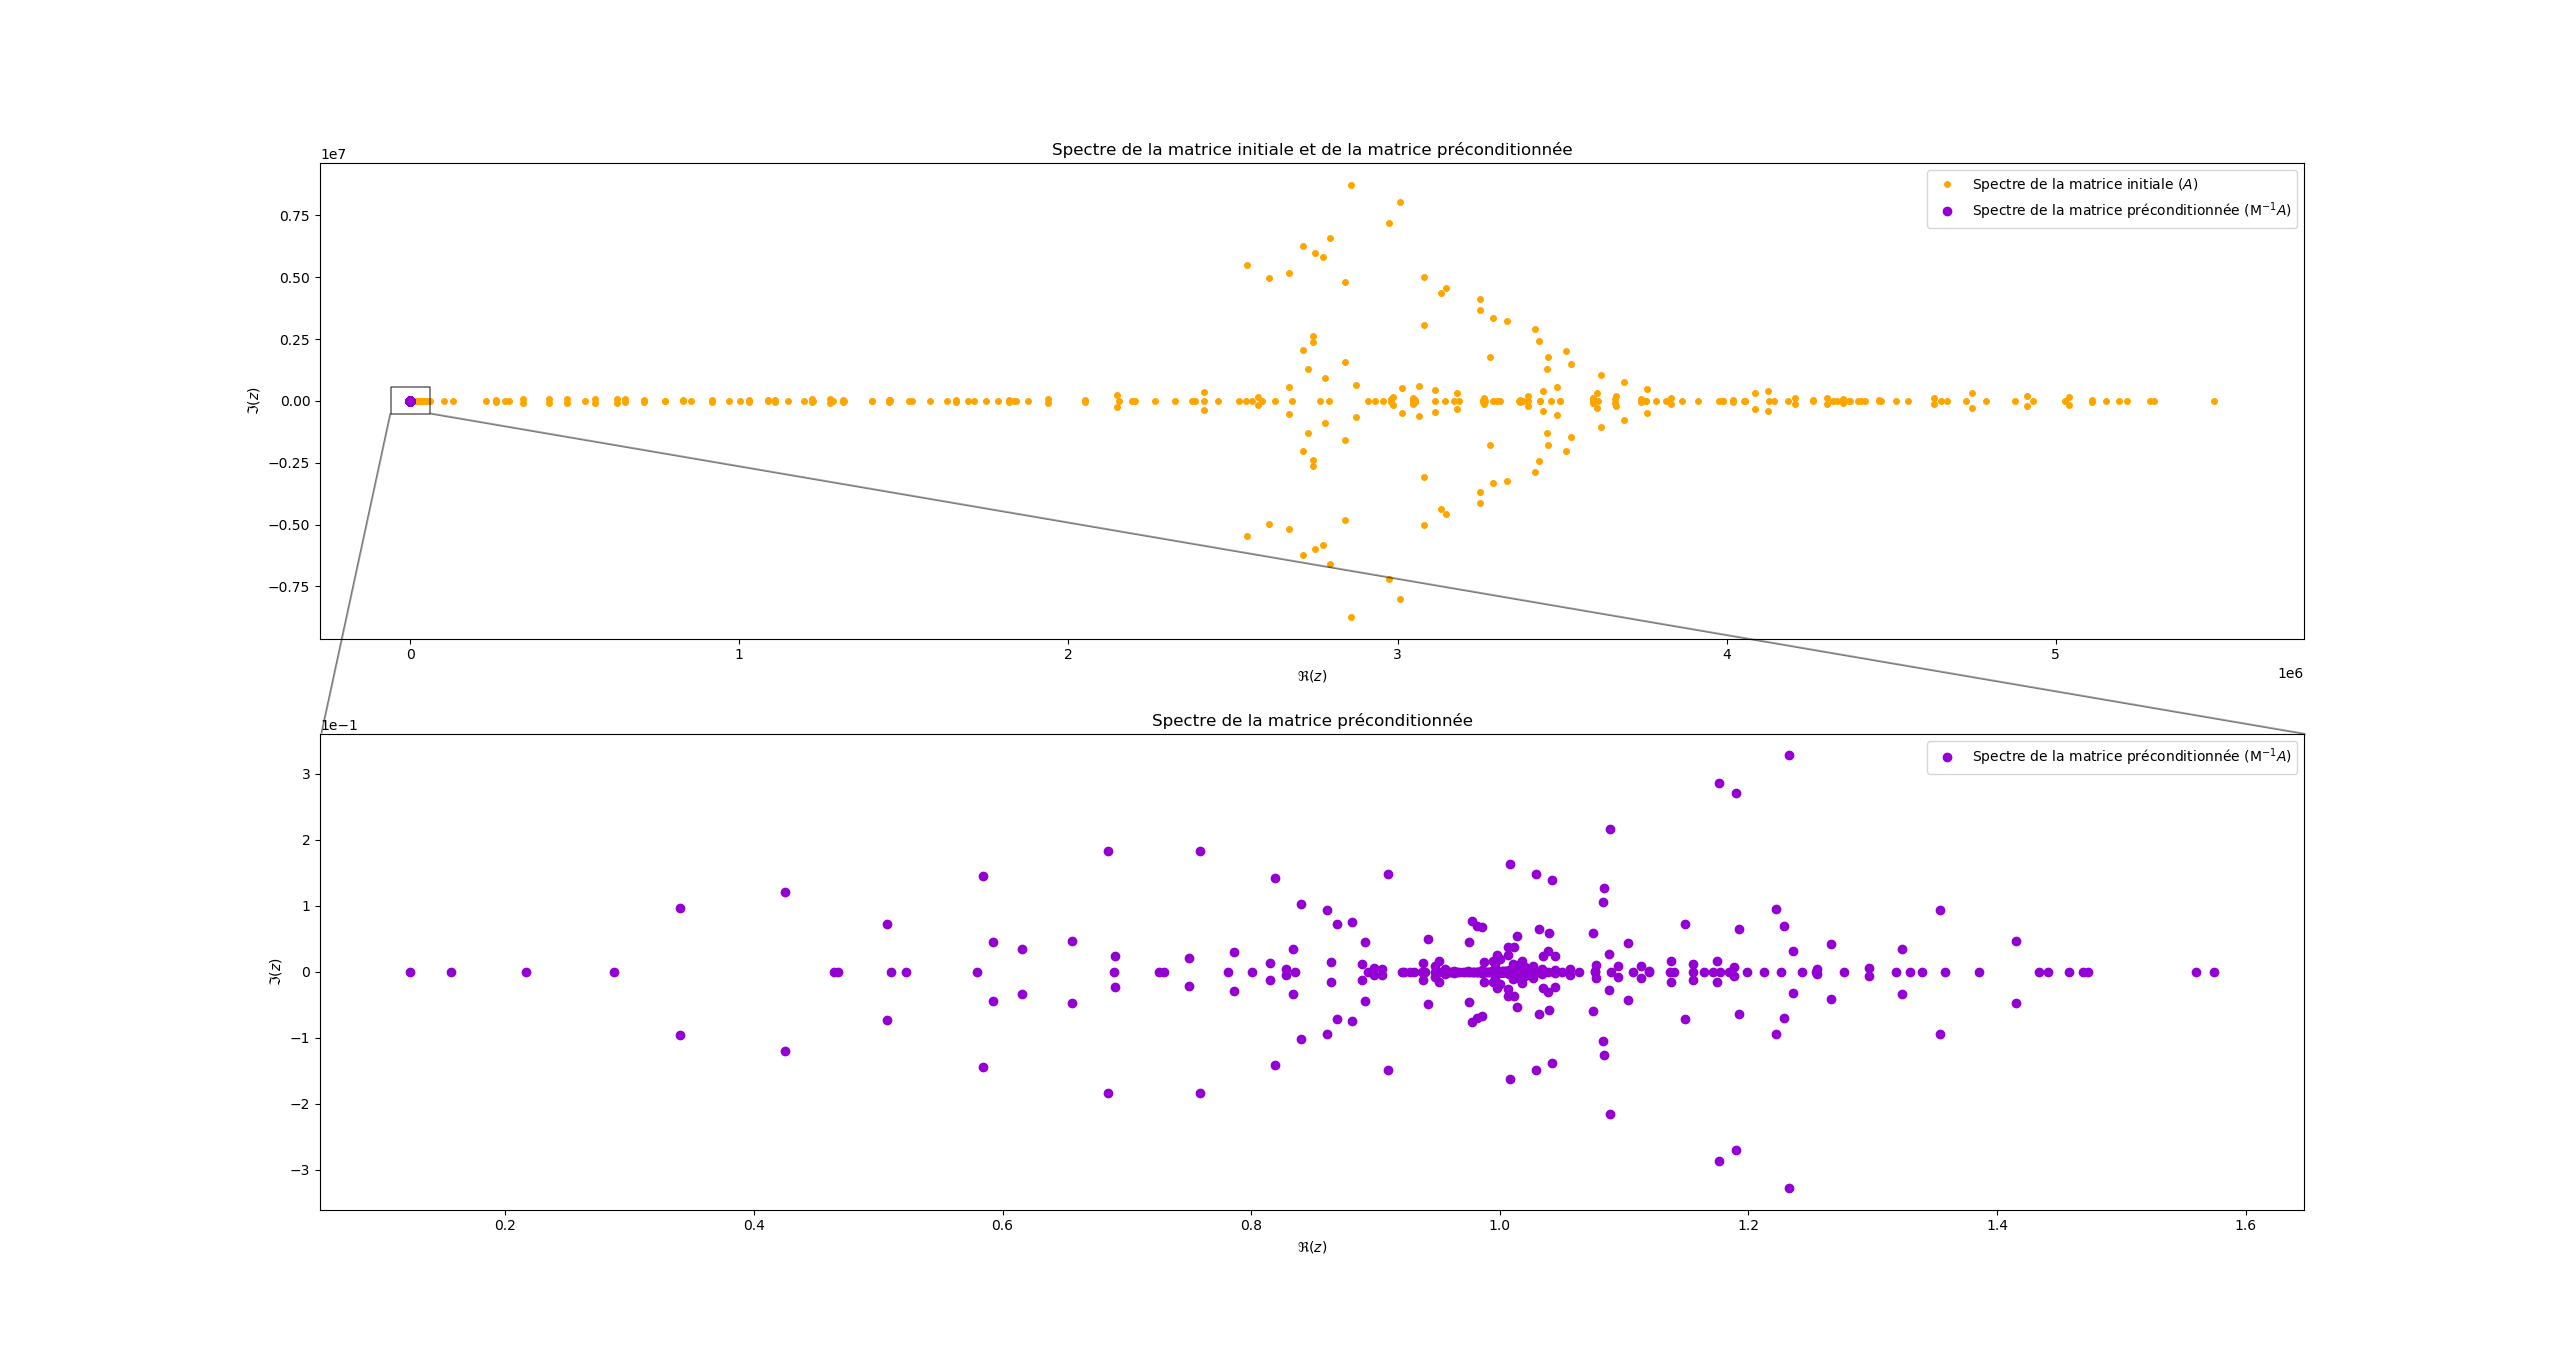
\includegraphics[width=.8\textwidth]{res/plots/spectrum.png}
	\caption{Spectre de $A$ et $M^{-1}A$}
	\label{fig:spectrum}
\end{figure}

\section{Convergence}
\label{sec:convergence}

Comme représenté sur la figure~\ref{fig:regimes}, on peut remarquer que le raffinement joue un rôle essentiel sur la rapidité de la convergence, le système étant plus grand, il met plus d'itérations pour converger. De plus la symétrie de la matrice (pas de vélocité) joue un rôle important sur la convergence de la norme du résidu puisque le nombre de conditionnement se voit plus petit que lorsque la matrice n'est pas symétrique, la convergence dépendant directement du nombre de conditionnement.

\begin{figure}[H]
	\centering
	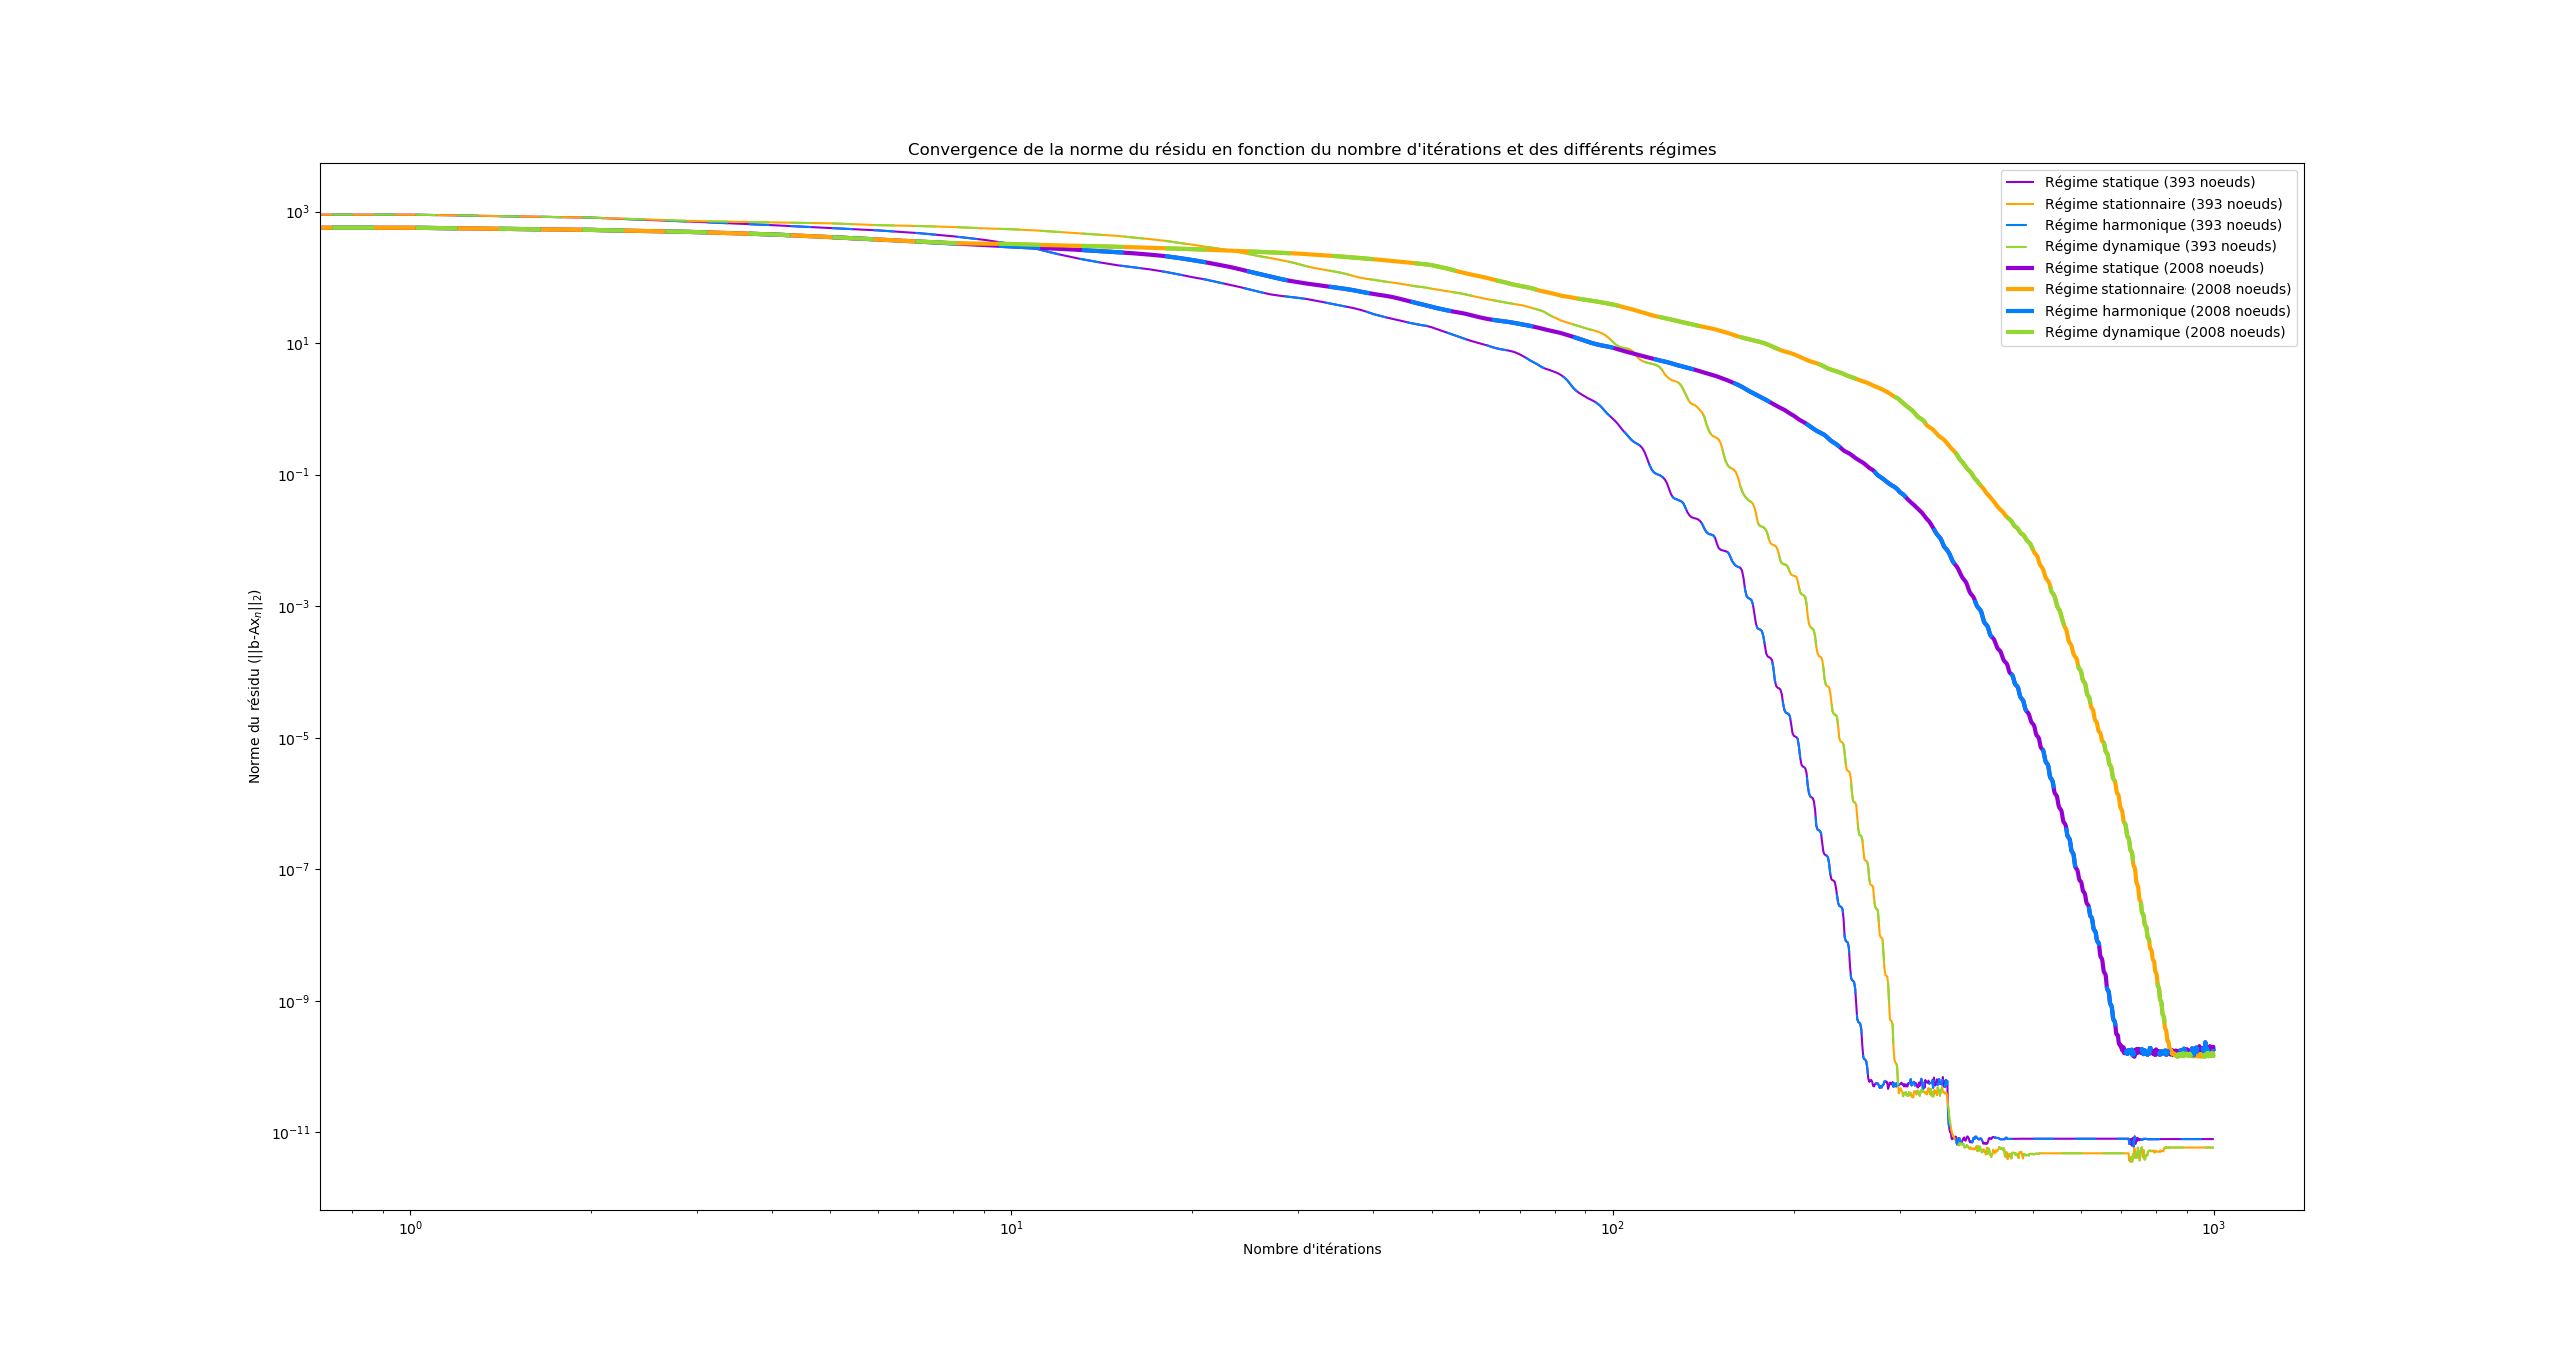
\includegraphics[width=.8\textwidth]{res/plots/regimes.png}
	\caption{Convergence de GMRES en fonction de la taille du système et du régime\label{fig:regimes}}
\end{figure}
\begin{center}
\begin{figure}[H]
\begin{tabular}{|c|c|c|c|c|c|c|}
	\hline
		\textbf{Itérations : $\boldsymbol{n}$} & 1 & 10 & 25 & 50 & 100 & 250 \\
	\hline
		$\boldsymbol{\norm{b-Ax_n}_2}$ & $1035.66$ & $373$ & $71.18$ &$18.31$ &$7.72\times 10^{-1}$ &$2.25\times 10^{-9}$ \\
	\hline
		$\boldsymbol{\norm{M^{-1}(b-Ax_n)}_2}$ & $2.13\times 10^{-3}$ & $6.32\times 10^{-5}$ &$5.10\times 10^{-8}$ &$8.07\times 10^{-18}$ &\textcolor{grey}{$1.09\times 10^{-17}$} &\textcolor{grey}{$1.35\times 10^{-17}$} \\
	\hline
\end{tabular}
\caption{Convergence avec et sans préconditionneur}
\label{tab:conv}
\end{figure}
\end{center}

\section{Code}
\label{sec:code}
\showCode{res/py/csrGMRES.py}
\showCode{res/py/csrILU0.py}
\end{document}
